\documentclass{standalone}
\usepackage{tikz}
\usetikzlibrary{mindmap}

\begin{document}

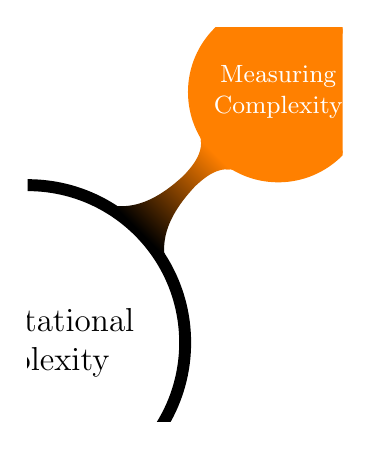
\begin{tikzpicture}[
  mindmap,
  every node/.style={concept, execute at begin node=\hskip0pt},
  root concept/.append style={
    concept color=black, fill=white, line width=1ex, text=black
  },
  text=white, grow cyclic,
  level 1/.append style={level distance=4.5cm,sibling angle=90},
  level 2/.append style={level distance=3cm,sibling angle=45}
]
\clip (0,-1) rectangle ++(4,5);
\node [root concept] {Computational Complexity}
  child [concept color=red] { node {Computational Problems}
    child { node {Problem Measures} } 
  }
  child [concept color=blue] { node {Computational Models}
    child { node {Turing Machines} }
  }
  child [concept color=orange] { node {Measuring Complexity}
    child { node {Complexity Measures} }
  }
  child [concept color=green!50!black] { node {Solving Problems}
    child { node {Exact Algorithms} }
  };
\end{tikzpicture}

\end{document}